\begin{frame}{Trouvons des négatives}
  \begin{enumerate}
    \item Écrivez trois questions qui pourraient susciter \gloss{elicit} des réponses négatives. Chaque question devrait susciter une négation différente, soit \lexi{pas}, \lexi{rien}, \lexi{jamais}, \lexi{personne}, \lexi{nulle part}, \lexi{aucun.e}, \lexi{plus}, \lexi{pas encore}, \lexi{ni...ni}.
    \item<2-> Pour chaque question, trouvez une personne dans la classe qui répond au négatif, et écrivez son nom à côté de la question. \emph{Répondez avec des phrases complètes!}
  \end{enumerate}
  \begin{center}
    \footnotesize
    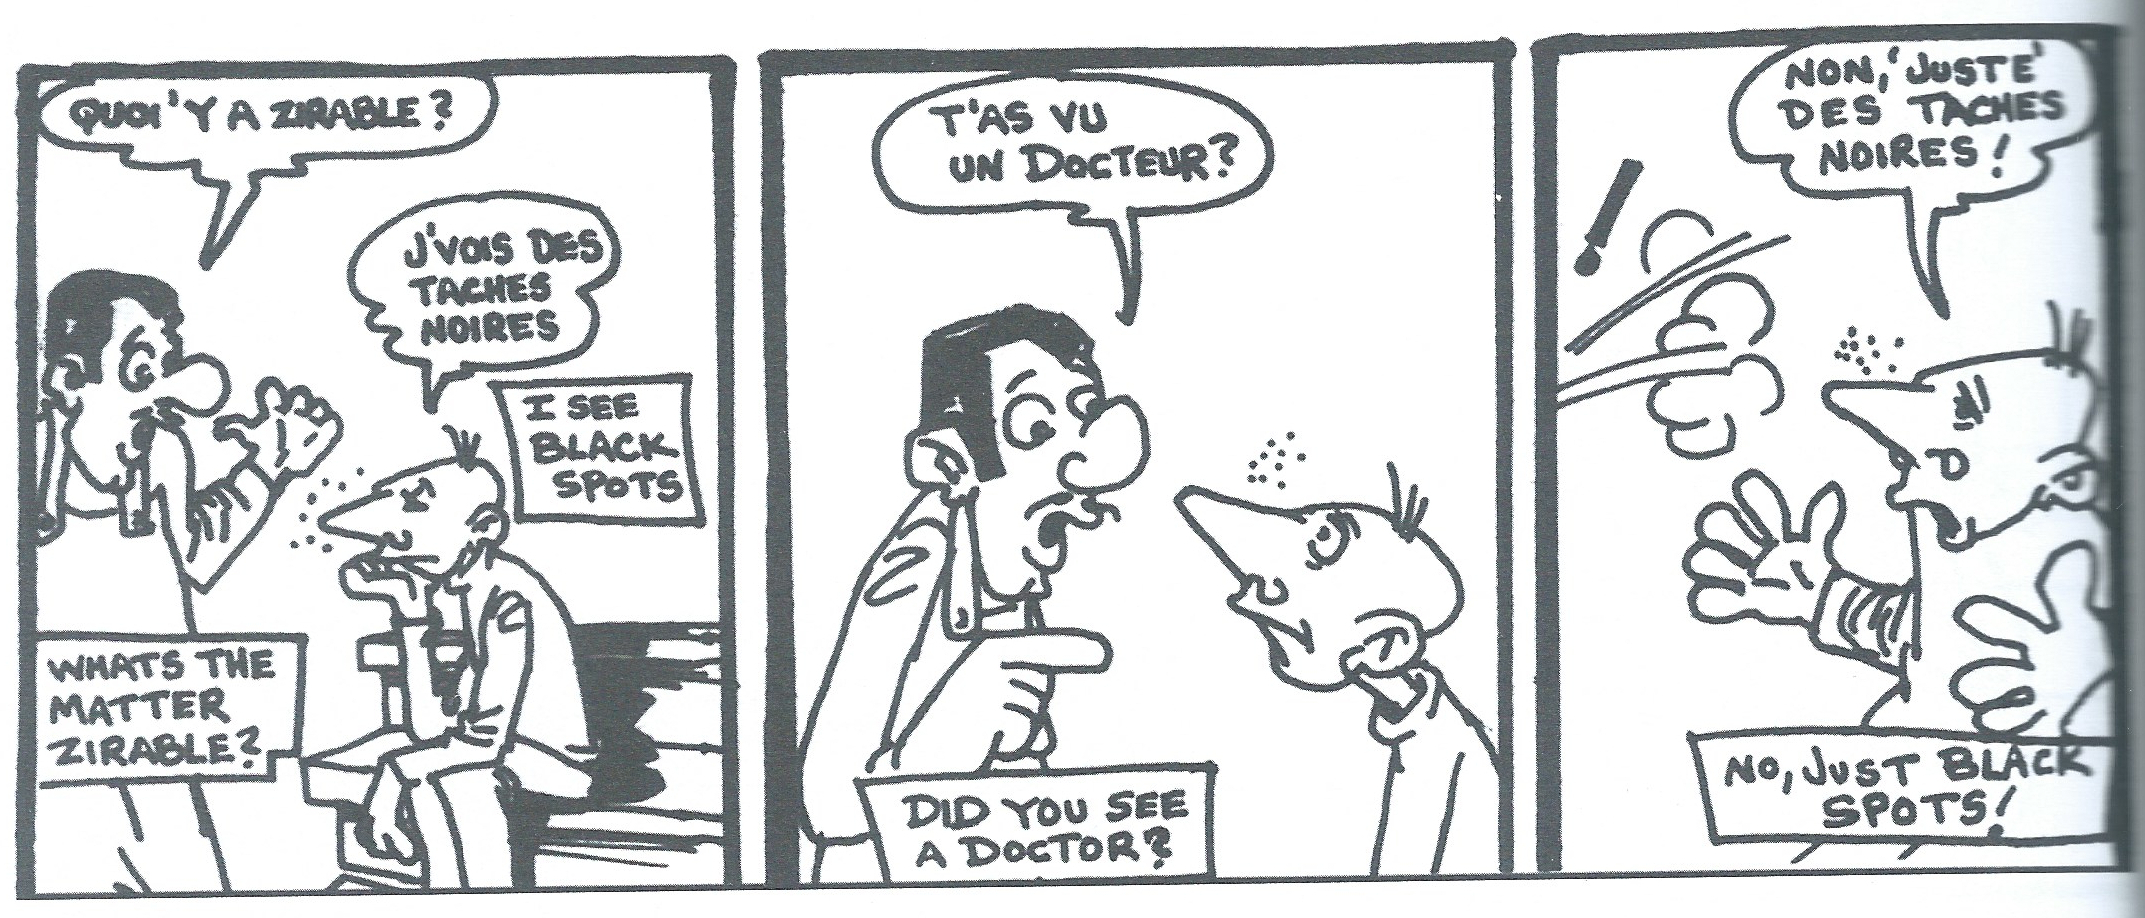
\includegraphics[scale=0.55]{bec_doux.jpeg} \\
    Bec Doux, 1971, bande dessinée de Louisiane
  \end{center}
\end{frame}